%
% graphisch3.tex
%
% (c) 2020 Prof Dr Andreas Müller, Hochschule Rapperswil
%
\begin{figure}
\centering
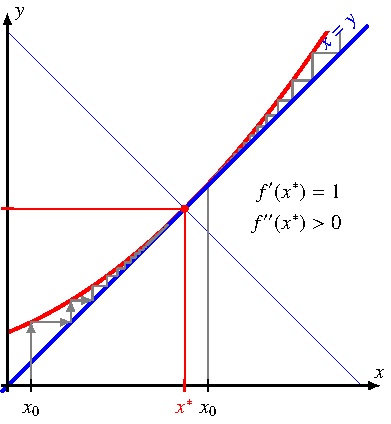
\includegraphics{chapters/10-arithmetik/figures/m1qp.pdf}
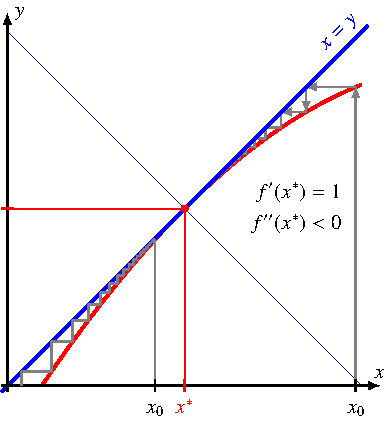
\includegraphics{chapters/10-arithmetik/figures/m1qn.pdf}
\caption{Konvergenzverhalten der Fixpunktiteration $x_{n+1}=f(x_n)$
in der Umgebung des Fixpunktes $x^*$ für $f'(x^*)=1$.
Falls $f''(x^*)>0$ konvergiert die Iteration sehr langsam
für einen Startwert $x_0>x^*$ falls $f''(x^*)>0$, divergiert
aber für einen Startwert $x_0>x^*$. 
Bei negativer zweiter Ableitung ist es umgekehrt.
\label{buch:figure:fixpunkt:abl1}}
\end{figure}
